\chapter{Experiment}
\section{Context Size}
\cite{Mikolov:13a} describe in their work how context size affects the type and quality of word vectors. One of the observations is that a smaller context size tend to capture syntactic similarity to a much better extent. As we increase the context size, vectors tend to capture more of semantic similarity.\\
\begin{figure}[ht]
\centering
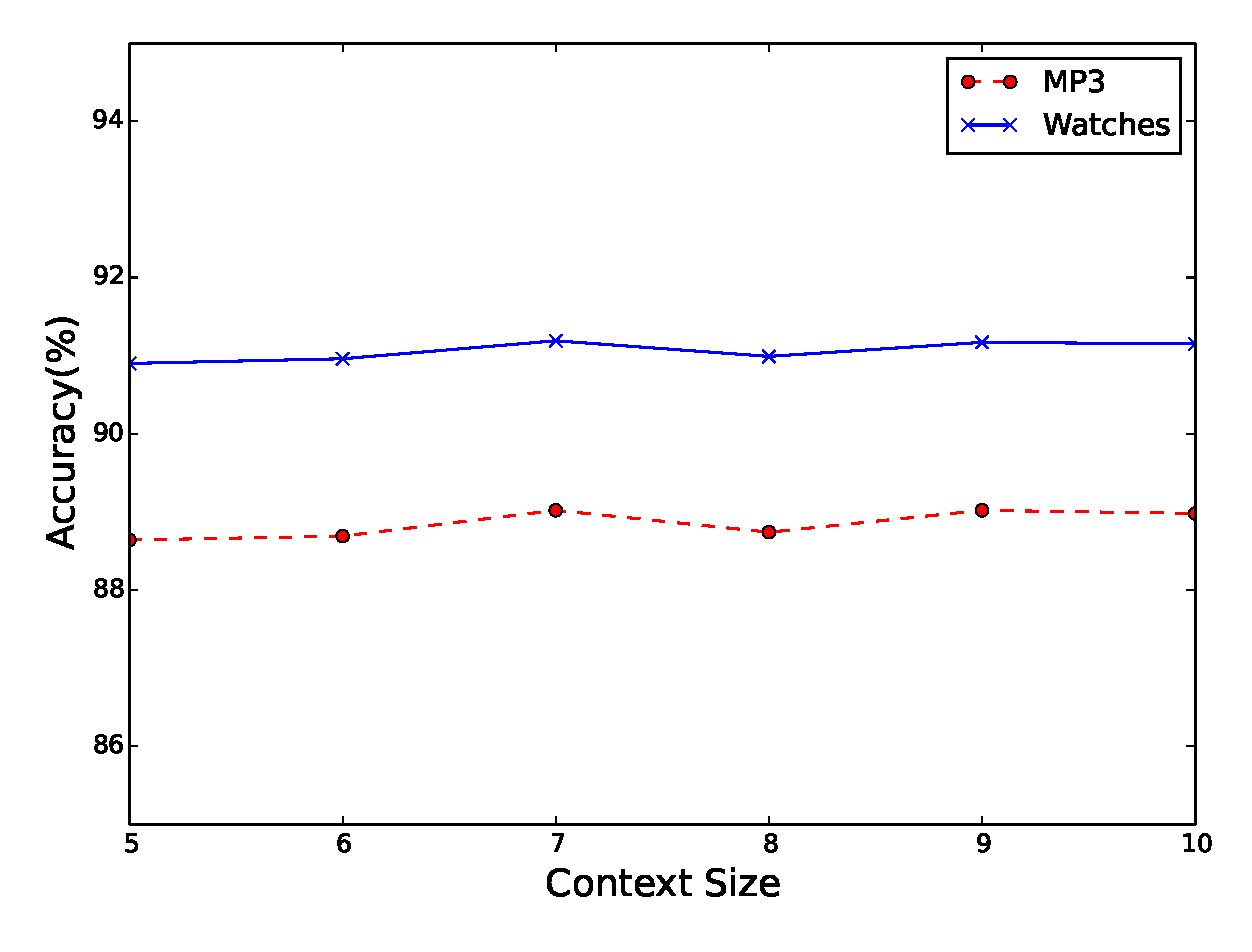
\includegraphics[width=140mm, height=110mm]{context_size.eps}
\caption{Variation of Accuracy with Different Context Size on Watches and MP3 Datasets. \label{fig:context_size}}
\end{figure}
We try to look how context size affects the accuracy on two amazon datasets, Watches and MP3.\\
Figure \ref{fig:context_size} depicts the accuracies obtained by varying the context size from 5 to 10. In both the cases, we find a peak at context size 7. There is an increase from 5 to 7 which denotes increase of context strength. As a result, we see increase in accuracies. Once the context size goes beyond a threshold, the semantic counterpart dominates which attains maximum at context size 10.\\
We also see that larger data size or training data affects the accuracy on test set. In this case, \emph{Watches} dataset is larger than \emph{MP3} dataset.\\

Figure \ref{fig:tsne_context} shows how the high dimensional representation changes when we change the context size. The embeddings were formed with context sizes 5 and 10 by training on Latest Wikipedia dump.
\section{SkipGram or CBOW}
SkipGram model tends to predict a context given a word whereas CBOW model predicts a word given a context. It seems intuitive and also from observation~\cite{Mikolov:13b} that SkipGram will perform better on semantic tasks and CBOW on syntactic tasks. We now try to evaluate how they differ on classification accuracies on the two datasets: \emph{Watches} and \emph{MP3}.
\begin{figure}[!ht]
\centering
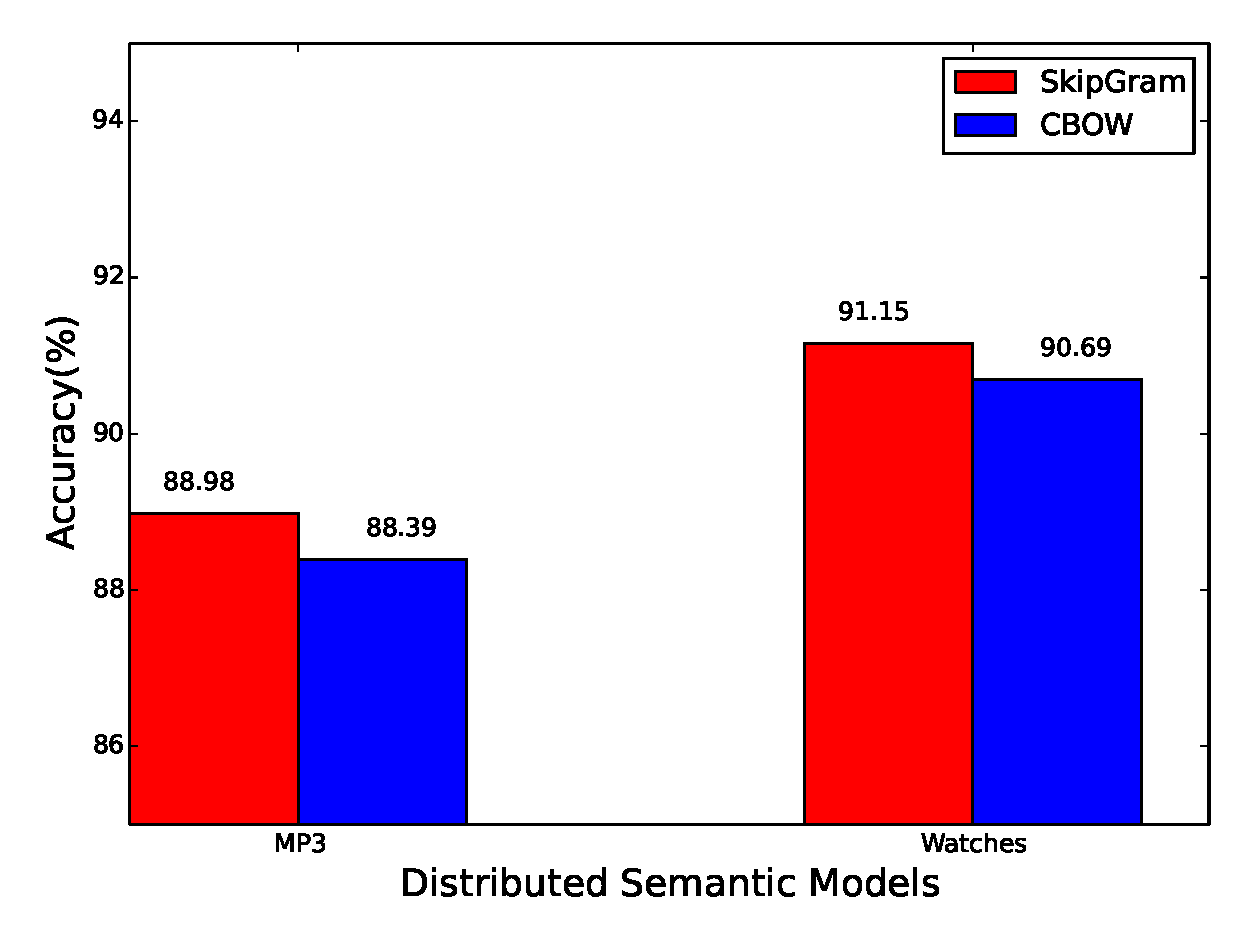
\includegraphics[width=140mm, height=110mm]{accuracy_sgcbow.eps}
\caption{Variation of Accuracy with Different Context Size on Watches and MP3 Datasets. \label{fig:accuracy_sgcbow}}
\end{figure}
Figure \ref{fig:accuracy_sgcbow} show that skipgram outperforms CBOW on sentiment classification task. It can be justified by the fact that sentiment inclination of a document is more oriented towards semantics of that document rather than just syntax and our results clearly demonstrate this fact.

A workflow defined as a graphic summary of the following has been depicted in Figure \ref{work_flow}.
We also trained our skip-gram model on Hindi Wikipedia text dump (approx. 290MB) containing around 24M words with 724K words in the vocabulary. This provided us with good embeddings due to larger size and contents from almost all domains.

The quality of word vectors can be evaluated by comparing them with words which are closer to them semantically and syntactically. This is usually done via cosine similarity.  Another evaluation can be done through tSNE~\cite{Maaten:08} which helps in visualization which maps each high-dimensional data point to a two or three-dimensional map. In our experiment, we took 5K words and plotted
them with tSNE (fig.~\ref{fig:5K_hindi_zoom}). 

\includepdf{tsne.pdf}

%\begin{figure}[ht!]
%\centering
%\includepdf[width=80mm]{tsne.pdf}
%\includegraphics[width=80mm]{tsne.pdf}
%\caption{t-SNE visualization of the top 5000 Hindi Words in high dimensional space.  (Magnify to see details).}
%\label{fig:5K_hindi_zoom}
%\end{figure}

Figure \ref{fig:5K_hindi_zoom} gives a closer look into few clusters which depicts the relation between words in high dimensional space. Figure \ref{fig:5K_hindi_zoom1} shows that words such as 
%{\dn mO\8{j}d} and {\dn uplND} 
are closer to each other but farther from words such as 
%{\dn \31EwyAdA} and {\dn aEDk}.

\begin{figure}[ht!]
    \centering
    \begin{subfigure}{.4\linewidth}
        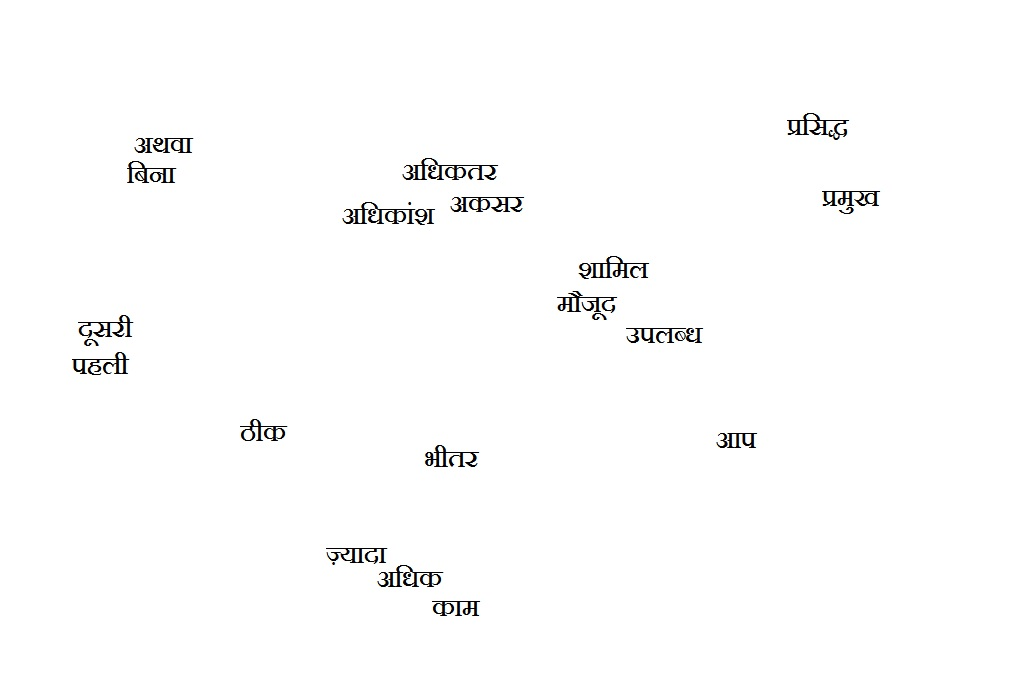
\includegraphics[scale=0.5]{5K_hindi_zoom1.eps}
        \caption{}
        \label{fig:5K_hindi_zoom1}
    \end{subfigure}
    \newline
    \begin{subfigure}{.4\linewidth}
        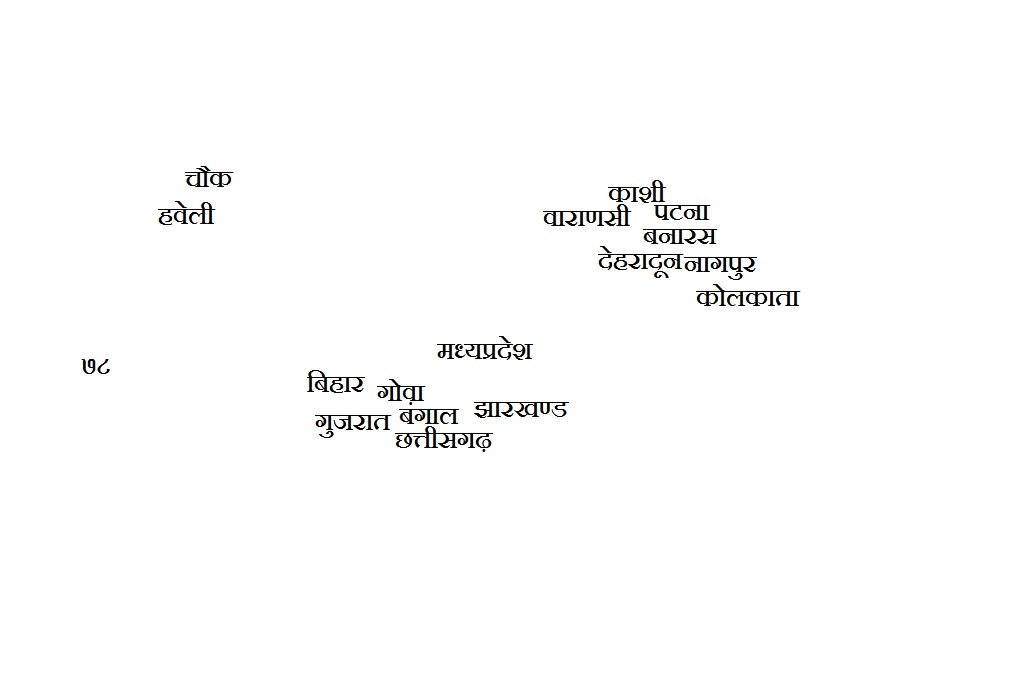
\includegraphics[scale=0.5]{5K_hindi_zoom2.eps}
        \caption{}
    \end{subfigure}
    \newline
    \begin{subfigure}{.4\linewidth}
        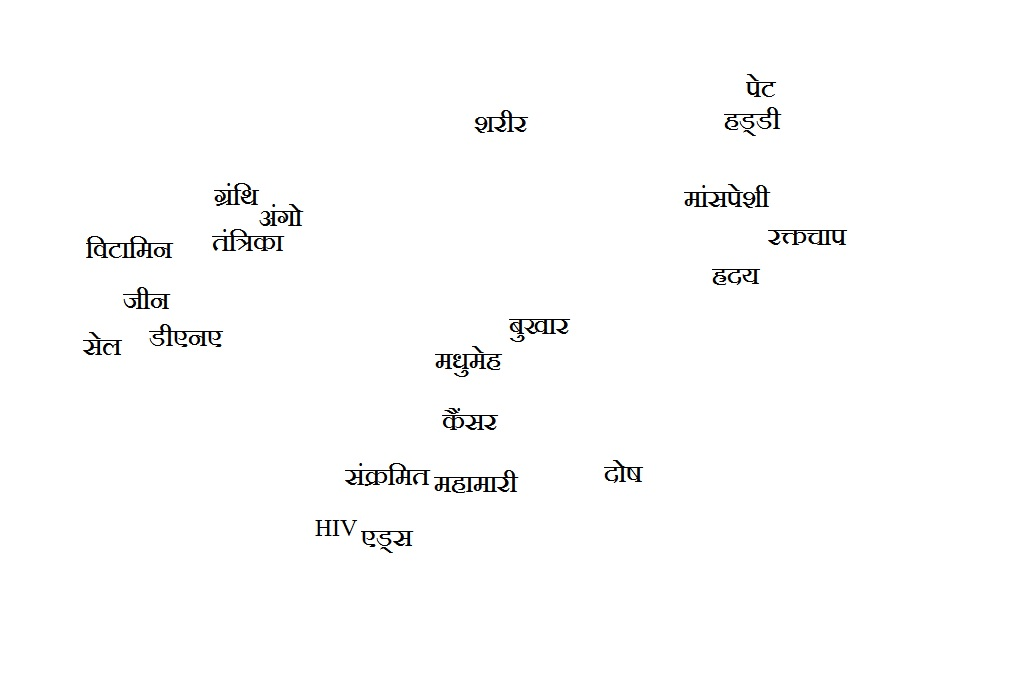
\includegraphics[scale=0.5]{5K_hindi_zoom3.eps}
        \caption{}
    \end{subfigure}
    \caption{A closer look at two clusters in the visualization showing a) quantity relations, b) locations and c) diseases.}
    \label{fig:5K_hindi_zoom}
\end{figure}

\subsection{Skip-Gram and \emph{tf-idf} based Word Vectors}
In this experiment, we first generated 300-dimensional word vectors by training skip-gram model on both review corpus. The context size was taken as 5. We then averaged-out word vectors for each document to create document vectors. This now acts as a feature set for that particular document.
We also created \emph{tf-idf} vectors for each document. This can be seen as a vector representation of that particular document. We then concatenated these document vectors with document vectors obtained after averaging-out word vector of each document. In this case, the dimension of each word vector obtained from skip-gram training was 500.

\subsection{Skip-Gram and \emph{tf-idf} based Word Vectors without stop-words}
In this experiment, we filtered out stop-words on the basis of their frequency in the corpus. Words which had very high or very low frequency were pruned as they had negligible contribution to the sentiment polarity of a document. This is a noise-reduction step and gives better results.
		\subsection{Tools/Libraries}
\begin{itemize}
	\item Eclipse: An Integrated Development Environment helped speed up the process of coding and its subsequent debugging.
	\item Python: Being a very common and widely used programming language, loads of  documentation and third party libraries are available.
	\item Scikit: Open source library built on NumPy, SciPy and matplotlib which contains simple and efficient tools for data mining and data analysis.
	\item Gensim: It is an open-source vector space modeling and topic modeling toolkit, implemented in the Python programming language, using NumPy, SciPy and optionally Cython for performance. It is specifically intended for handling large text collections, using efficient online algorithms.
\end{itemize}

		\subsection{System Requirements}
		The code and tests have been successfully run on the following configuration. Any system with a configuration equal or higher than this should be able to do the job faster.
\begin{itemize}
	\item RAM: 16GB; fails to run on 8GB, due to the high amount of in memory data.
	\item CPU: Intel Core i7, 4th Generation; have used all 8 virtual cores with hyper-threading, with lower CPU, processes would take longer to complete.
	\item HDD: 280GB dedicated; Million Song Dataset is the only component using considerable persistent memory. Storing user history and codes consume very minimal data storage (in MBs).
\end{itemize}
		
		\subsection{Optimizations}
\begin{itemize}
	\item Parallelization: Since, gathering data for every user is fairly independent of each other, these tasks have been implemented in parallel. Also, during the recommendation, once the set of similar users have been collected, suggesting songs per user can again be done in parallel. 16 threads has been found to be the optimal for speed on a CPU with 8 virtual cores (2 hyperthreads per core).
	\item On-Demand: Most songs from the dataset would not be required for recommending, and might consume some valuable runtime. The songs are loaded in the memory at the first missed access. This not only ensures faster runtime but also a lower comsumption of physical memory.
	\item Load Minimal Data Efficiently: Only song data like \emph{loundess}, \emph{tempo} and \emph{popularity} that is required for recommending is loaded into memory. This data is stored in a serialized JSON format. This lightens the overhead of high-level data structures.
	\item Prevent File Access: Each song's information in the million song dataset is stored away in a separate file for each. This heightens the overhead of several files being opened and closed at runtime. Also, there is a limit imposed by the OS to the number of files that can remain open at any given point of time. Thus, only the required information has been extracted, compressed into a serialized format and loaded in memory on an on-demand basis.
\end{itemize}
	
		\subsection{Complications}
\begin{itemize}
	\item Last.FM API: The API is not very robust when multiple calls are made in a short span of time. Several of the calls tend to get failed resulting in the obtained history being corrupted. This restricts the use of multi-threading to fetch user data, which would have improved the runtime significantly.
\end{itemize}
	
		\subsection{Improvements}
\begin{itemize}
	\item Distributed Systems: It gives advantages in terms of more number of CPUs and thus more threads at work, enabling to reduce the runtime considerably. Also, the Last.FM API finds itself in a bit of fix when several calls are being made at the same time from the same computer; this also then can be relieved. This would also enable load balancing the recommendation requests.
	\item NFS: Using an NFS over a local network could shared the dataset and user histories across all the involved machines.
\end{itemize}

	\section{Work Flow Summary}
		\begin{figure}[h!]
			\centering
			
\includegraphics[width=15cm]{iitkblue.eps}
			\caption{Work Flow\label{work_flow}}
		\end{figure}
			
